\documentclass[11pt, a4paper,svglistings,oneside]{book}
\usepackage{a4wide}
\usepackage[USenglish]{babel}
\usepackage{graphicx}
\usepackage{float}
%\usepackage{mathtools}

\setcounter{secnumdepth}{3}   
\setcounter{tocdepth}{3}   

\usepackage[toc,page]{appendix}

\usepackage{hyperref}
\hypersetup{
    colorlinks,
    citecolor=black,
    filecolor=black,
    linkcolor=black,
    urlcolor=black
}

\usepackage{fullpage}
\usepackage{listings}
\usepackage{xcolor}
\usepackage{textcomp}

\usepackage[explicit]{titlesec}
\usepackage{lmodern}
\usepackage{lipsum}

\usepackage[USenglish]{babel}
\usepackage[square]{natbib}

\newlength\chapnumb
\setlength\chapnumb{4cm}

\titleformat{\chapter}[block]
{\normalfont\sffamily}{}{0pt}
{\parbox[b]{\chapnumb}{%
   \fontsize{120}{110}\selectfont\thechapter}%
  \parbox[b]{\dimexpr\textwidth-\chapnumb\relax}{%
    \raggedleft%
    \hfill{\LARGE#1}\\
    \rule{\dimexpr\textwidth-\chapnumb\relax}{0.4pt}}}
\titleformat{name=\chapter,numberless}[block]
{\normalfont\sffamily}{}{0pt}
{\parbox[b]{\chapnumb}{%
   \mbox{}}%
  \parbox[b]{\dimexpr\textwidth-\chapnumb\relax}{%
    \raggedleft%
    \hfill{\LARGE#1}\\
    \rule{\dimexpr\textwidth-\chapnumb\relax}{0.4pt}}}

\graphicspath{ {./images/} }

\usepackage[labelfont=bf]{caption}
\usepackage{pdfpages}

\begin{document}

\begin{titlepage}

\newcommand{\HRule}{\rule{\linewidth}{0.5mm}}

\center

%----------------------------------------------------------------------------------------
%	HEADING SECTIONS
%----------------------------------------------------------------------------------------

\textsc{\LARGE VRIJE UNIVERSITEIT BRUSSEL}\\[1.5cm] 
\textsc{\Large Faculty of Science and Bio-Engineering Sciences}\\[0.5cm] 
\textsc{\large Departement of Computer Sciences}\\[0.5cm] 

%----------------------------------------------------------------------------------------
%	TITLE SECTION
%----------------------------------------------------------------------------------------

\HRule \\[0.7cm]
{ \huge \bfseries Web Engineering Assignment 3: Report}\\[0.4cm] 
\HRule \\[1.5cm]
 
%----------------------------------------------------------------------------------------
%	AUTHOR SECTION
%----------------------------------------------------------------------------------------

\begin{minipage}{0.4\textwidth}
\begin{flushleft} \large
\emph{Authors:}\\
Laurent \textsc{De Wilde} \\
Mathias \textsc{Alame}
\end{flushleft}
\end{minipage}
~
\begin{minipage}{0.4\textwidth}
\begin{flushright} \large
\emph{Professor:} \\
Prof. Dr. Sven \textsc{Castelyn}

\emph{Assistant:} \\
Msc. Pejman \textsc{Sajjadi}
\end{flushright}
\end{minipage}\\[4cm]

%----------------------------------------------------------------------------------------
%	DATE SECTION
%----------------------------------------------------------------------------------------

{\large \today}\\[3cm]

%----------------------------------------------------------------------------------------
%	LOGO SECTION
%----------------------------------------------------------------------------------------


\includegraphics[width=2.3in]{vub_schild.jpg}\\[4cm] 
 
%----------------------------------------------------------------------------------------




\end{titlepage}

 \frontmatter

\tableofcontents

\listoffigures

\chapter{Preface}

This document describes the development process of the website ``Date4Life'' created by Laurent De Wilde and Mathias Alame. \\
The website has been created by using WSDM - Web Semantic / Site Design Method, an audience driven design method for Web Applications \citep{WSDM2}. \\
This design method consists of five major phases and the output of each phase serves as the input for the following (next) phase. Subsequently, each phase consists of multiple sub-phases, which are described extensively in this document.

\mainmatter

\chapter{Mission statement specification}

In the mission statement specification, the purpose, the subject (topics) and the targeted users of the web site are specified \citep{WSDM1}. The mission statement serves as a starting point for the design process. It will set boundaries for the design by identifying purposes of the website \citep{WSDM2, WSDM3}. \\
The target users of the website are the users that will use and interact with the website. The subject must fulfill the purpose of the website and must be adapted for the target users \citep{WSDM2}. \\
After the completion of the design process, the mission statement is used to verify if the goals of the website have been fulfilled \citep{WSDM3}.

\section{Mission statement}

The purpose of the dating site is to make sure that singles and couples, regardless of their age, gender or sexual interest, find new friends or the love or their life by displaying user profiles and detailed information about a possible suitable opponent and to provide search functionality, a private chat system and liking other users.

\subsection{Purpose}

Finding friends or the love or their live.

\subsection{Target audience}

Singles who want to participate in a relationship, or people currently involved in a relationship who are looking for friendship.

\subsection{Subject}

User profiles

\chapter{Audience modeling}

In the audience modeling phase, the target audiences / users defined in the mission statement phase are refined into audience classes \citep{WSDM2}. In these classes, the users are grouped that have the same functional and information requirements. Users with additional requirements form audience subclasses \citep{WSDM3}. \\
So the audience classes form a hierarchy, where the most general class - the visitor class, is at the top of the hierarchy - that is, the common requirements for all visitors. For each additional level, more specific requirements are formulated \citep{WSDM3}.

\section{Audience classification}

These are the different audience classes for the website:
\begin{itemize}
\item \textbf{Visitors:} the most general class. They can only search for user profiles and see some basic information about the last members that logged in.
\item \textbf{Registered users:} have the same privileges as the visitors + much more functionality such as the possibility to login and send messages.
\item \textbf{Singles:} have the same privileges as the registered users + much more functionality such as the liking other users, request friendships with other users and to send attentions.
\item \textbf{Administrators:} have the same privileges as the registered users + they are able to see all information about all the users and can manage any user, including disabling and deleting a user.
\end{itemize}

\subsection{Audience class visitors}
\label{sec:visitorclass}
This is the most general audience class and they have the least number of privileges. They can only search for existing members - the so-called ``singles'', register a new account or login using an existing user account. Additionaly, information is shown about the last 10 members that have logged in.

\paragraph{Information requirements}

Information about the top 10 members they searched for and information about the last 10 members that logged in. In both cases, the information includes nickname, age, location, picture and gender.

\paragraph{Functional requirements}

\begin{itemize}
\item Visitors should be able to search based on age, range, location and gender.
\item Visitors should see the nickname, age, location, picture and gender of the last 10 members that logged in.
\item Visitors should be able to login, specifying a username and a password.
\item Visitors should be able to register a new account, thereby providing a nickName, password, email address, location, gender, interest and a free description.
\end{itemize}

\paragraph{Usability \& navigational requirements}

\begin{itemize}
\item The user should be able to quickly search for members.
\item The search results should easily be readable in a comprehensive way.
\item It should clearly be visible how to login.
\end{itemize}

\subsection{Audience class registered users}

The ``registered users'' audience class is a subclass of the visitors user class. They have extra privileges and functionality: they are able to edit their personal profile, to search for users, to send them private messages, to logout and to terminate their account. \\
The ``registered user'' class is a superclass for the ``singles'' and ``administrator'' audience classes.

\paragraph{Information requirements}

\begin{itemize}
\item Detailed personal information 
\item Detailed information about other users' profiles.
\end{itemize}

\paragraph{Functional requirements}

\begin{itemize}
\item The users should be able to change, add or delete any information on their personal profile.
\item The users should be able to search for other users, based on the profile information.
\item The user profiles of other members can be seen by the users.
\item The users should be able to communicate to other registered users by sending them private messages.
\item The users should be able to log out and terminate their account.
\end{itemize}

\paragraph{Usability \& navigational requirements}

\begin{itemize}
\item The user should be able to quickly search for members.
\item The returned search results should easily be readable in a comprehensive way.
\end{itemize}

\subsection{Audience class singles}
\label{sec:singlesclass}
The ``singles'' audience class is the actual target audience of the web application. They have all the functionality and privileges of the ``registered users'' audience class and in addition, very much more functionality is availabe. For example, they can put messages on another user's wall, delete messages on their own wall, like users, and so on\ldots.\\

\paragraph{Information requirements}

\begin{itemize}
\item Detailed personal information 
\item Detailed information about other users' profiles.
\item Information on private messages.
\item Information on updates of liked user profiles.
\item Information on sent intentions.
\end{itemize}

\paragraph{Functional requirements}

\begin{itemize}
\item The users should be able to put messages on any user's wall, answer to a message on their own wall or deleting messages from their wall.
\item The users should be able to communicate to other registered users by sending them private messages.
\item The users should be able to ``like'' other users and should be able to manage their ``liked'' list.
\item The users should be notified in case of profile updates of their ``liked users''.
\item The users should be able to send another user an attention. These attentions should be the following:
	\begin{itemize}
	\item A bouquet of flowers
	\item A handshake
	\item A Smiley
	\item A kiss
	\item A tap on the back
	\item A thumbs up
	\item A bottle of wine
	\end{itemize}
\item The users should be informed about a received attention and should be able to return the favor.
\item The users should be able to message with randomly selected users, based on the selected gender and age.
\end{itemize}

\paragraph{Usability \& navigational requirements}

\begin{itemize}
\item Updates about other ``liked'' users should be eye-catching.
\item Attentions received from other users should clearly be visible.
\item \ldots
\end{itemize}

\subsection{Audience class administrators}

The ``administrator'' audience class is a subclass of the ``registered users'' class. The have the same privileges as them, but can browse all user profiles, send a message to any user, as well as deleting any user account.

\paragraph{Information requirements}

Information about users and information about blocked and reported users.

\paragraph{Functional requirements}

\begin{itemize}
\item The users should be able to browse through al user profiles.
\item The user should receive a message when another user blocks or reports a user.
\item The users can send a message to any other user.
\item The users can block, disable or delete any user account.
\end{itemize}

\paragraph{Usability \& navigational requirements}

\begin{itemize}
\item No additional usability requirements.
\end{itemize}

\section{Audience class hierarchy}

The figure below depicts the audience class hierarchy. \\

\noindent\begin{minipage}{\textwidth}
    \centering
   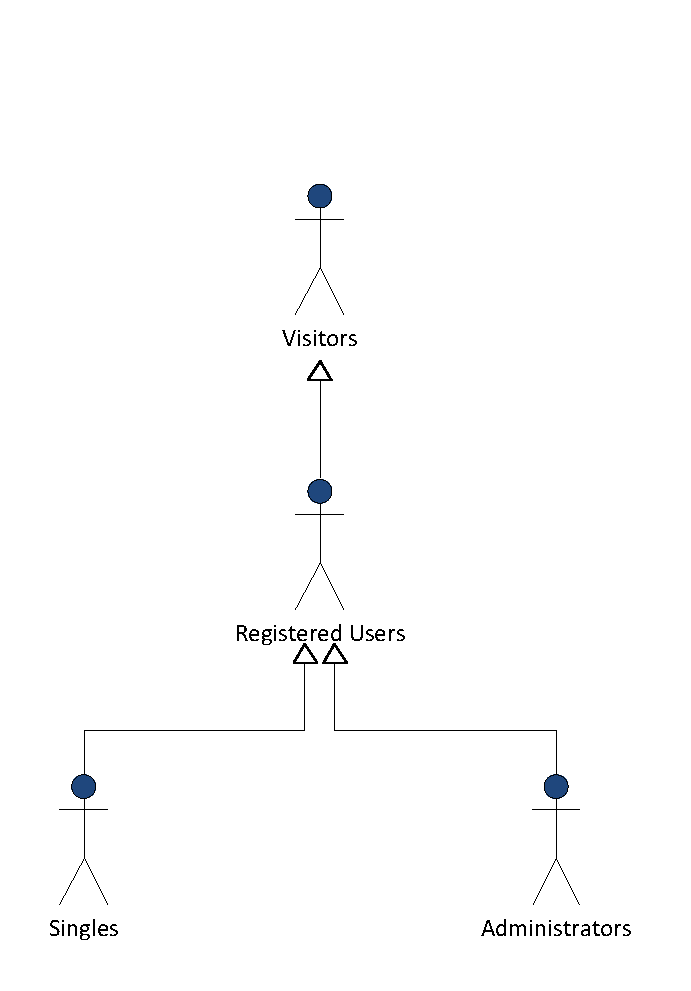
\includegraphics[scale=1]{Users3.pdf}
 \captionof{figure}[Audience class hierarchy]{Audience class hierarchy. \texttt{Visitors} is the superclass from which the subclasses \texttt{Registered Users} extends. This class, in his turn, is superclass for the  \texttt{Singles} and \texttt{Administrators} classes.}
\end{minipage}

\section{Audience Characterization}

The target users of the Date4Life website are quite a broad audience. There all have their own local language, but at the same time, they are able to communicate in English as well. \\
Also, the experiece with the Web may vary; some have much experience, while other do not. The age varies as well; some visitors are elderly adults, while others are young adults. \\
Finally, not all audience may be familiar with the concept of a dating site. Furthermore, it is assumed that administrators have more experience with the WWW in comparision to other users as well as more technical experience in general.

\subsection{Audience class Visitors}

\begin{itemize}
\item All ages starting from 18 years old.
\item Experience with a dating site may vary.
\item Are able to communicate in English.
\item Familiarization / experience with a dating site may vary.
\item Familiarization / experience with the WWW in general may vary.
\end{itemize}

\subsection{Audience class Registered Users}

\begin{itemize}
\item All ages starting from 18 years old.
\item Experience with a dating site may vary.
\item Are able to communicate in English.
\item Familiarization / experience with a dating site may vary.
\item Familiarization / experience with the WWW in general may vary.
\end{itemize}

\subsection{Audience class Singles}

\begin{itemize}
\item All ages starting from 18 years old.
\item Experience with a dating site may vary.
\item Are able to communicate in English.
\item Familiarization / experience with a dating site may vary.
\item Familiarization / experience with the WWW in general may vary.
\end{itemize}

\subsection{Audience class Administrators}

\begin{itemize}
\item All ages.
\item May be unfamiliar with a dating site.
\item Are able to communicate in English.
\item Have experience with the WWW varying from above-average to great.
\item Have an above-average technical background and experience.
\end{itemize}

\subsection{Conclusion}

From the audience class characterizations, one can conclude that all audience classes are able to communicate in English and thus there is no need to make any audience class variants.

\chapter{Conceptual Design}

In the previous phases, the information-, functional-, navigational- and usability requirements as well as the characteristics of the different audience classes have been identified. \\
In the third phase - the conceptual design phase, the requirements mentioned above are turned into formal descriptions, which can be used in a later phase to generate the website. \\
This phase consists of two sub-phases: the task modeling phase and the navigational design phase.

\section{Task Modeling}

\subsection{Audience class Visitors}
$\;$ \\
\underline{Requirement:} ``The users should be able to login, specifying a username and password.''. \\ \\
\underline{Task:} Login with a username and password. \\
When a user wants to login, he or she can enter their credentials, being the username and the password. After submitting, the system validates the provided credentials and redirects the user to the main page. \\ \\
\underline{Decomposition:}
\begin{itemize}
\item Enter the username.
\item Enter the password.
\item Submit the filled in data.
\item Process the authentication.
\item Redirect to the main page.
\end{itemize}
\noindent\begin{minipage}{\textwidth}
    \centering
   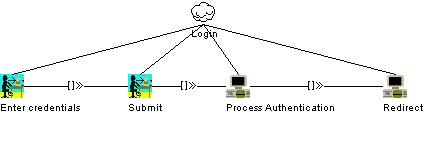
\includegraphics[width=\textwidth]{CTT_Login.png}
 \captionof{figure}[Login CTT]{CTT to login using a username and password.}
\end{minipage}
$\;$ \\ \\
%----------------------------------------------------------------------------------------------------------
\underline{Requirement:} ```A visitor should be able to create an account.'' \\ \\ 
\underline{Task:} Register new user. \\
A visitor needs to be able to create a new user account on the website. I.e., he needs to be able to register himself. The following information is required upon registration: date of birth, nickname, password, email address, location, interest and a free description. \\ \\
\underline{Decomposition:}
\begin{itemize}
\item Enter the credentials.
\item Register account.
\item Redirect to profile page.
\end{itemize}
\noindent\begin{minipage}{\textwidth}
    \centering
   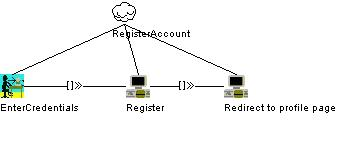
\includegraphics[width=\textwidth]{CTT_Register.png}
 \captionof{figure}[Register CTT]{CTT to register new user account.}
\end{minipage}
$\;$ \\ \\
%----------------------------------------------------------------------------------------------------------
\underline{Requirement:} ``Information about the top 10 members they searched for.'' \\ \\
\underline{Task:} Show information about the top 10 members that match a search query. \\
When a non-logged in user enters a search query, the nickname, location, gender, age and picture have to be displayed in any order. \\ \\
\underline{Decomposition:}
\begin{itemize}
\item Enter the nickname of the user.
\item Enter the age of the user.
\item Enter the location of the user.
\item Enter the gender of the user.
\item Show the top 10 matches.
\end{itemize}
\noindent\begin{minipage}{\textwidth}
    \centering
   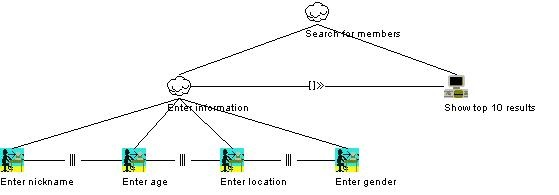
\includegraphics[width=\textwidth]{CTT_Search.png}
 \captionof{figure}[Search CTT]{CTT search for members and returning the top 10 results.}
\end{minipage}
$\;$ \\ \\
%----------------------------------------------------------------------------------------------------------
\underline{Requirement:} ``Visitors should be able to search based on age, range, location and gender.'' \\ \\
\underline{Task:} Search on age, range, location and gender. \\ \\
\underline{Decomposition:}
\begin{itemize}
\item Enter the age of the user.
\item Enter the range of the user.
\item Enter the location of the user.
\item Enter the gender of the user.
\item Display the results.
\end{itemize}
\noindent\begin{minipage}{\textwidth}
    \centering
   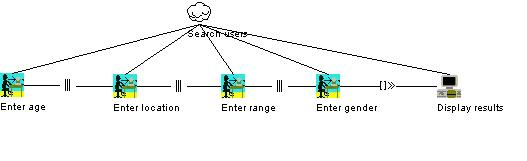
\includegraphics[width=\textwidth]{CTT_Search_2.png}
 \captionof{figure}[Visitor search CTT]{CTT search for membersbased on age, range, location and gender and returning the top 10 results.}
\end{minipage}
$\;$ \\ \\
%----------------------------------------------------------------------------------------------------------
\underline{Requirement:} ``information about the last 10 members that logged in.'' \\ \\
\underline{Task:} Show information about the last 10 members that logged in. \\
The nickname, location, gender, age and picture of the 10 last logged in members have to be displayed in any order. \\ \\
\underline{Decomposition:}
\begin{itemize}
\item Display the nickname of the member.
\item Display the location of the member.
\item Display the gender of the member.
\item Display the age of the member.
\item Display the picture of the member.
\end{itemize}
\noindent\begin{minipage}{\textwidth}
    \centering
   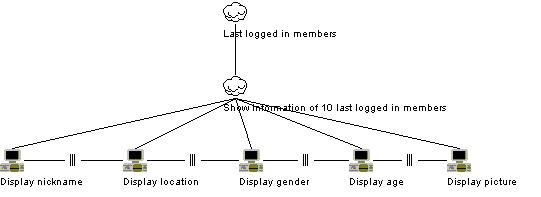
\includegraphics[width=\textwidth]{CTT_Members.png}
 \captionof{figure}[Last logged in members CTT]{CTT for showing the last 10 members that logged in.}
\end{minipage}
%----------------------------------------------------------------------------------------------------------
\subsection{Audience class Registered Users}
%----------------------------------------------------------------------------------------------------------
$\;$ \\
\underline{Requirement:} ``The registered users should be able to change any information on their personal profile.'' \\ \\
\underline{Task:} Change information of the personal profile. \\
When a user wants to change any information of their personal profile, he or she should first navigate to the profile information, edit the desired information and save the changes made. \\ \\
\underline{Decomposition:}
\begin{itemize}
\item Access the personal profile.
\item Edit the nickname.
\item Edit the age.
\item Edit the location.
\item Edit the gender.
\item Edit the picture.
\item Commit the changes.
\end{itemize}
\noindent\begin{minipage}{\textwidth}
    \centering
   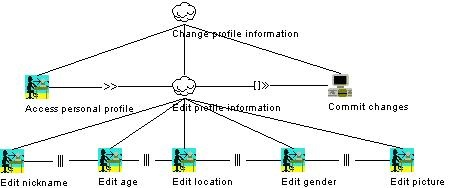
\includegraphics[width=\textwidth]{CTT_Profile.png}
 \captionof{figure}[Edit personal profile CTT]{CTT to change information on the personal profile.}
\end{minipage}
$\;$ \\ \\
%----------------------------------------------------------------------------------------------------------
\underline{Requirement:} ``The registered users should be able to add any information on their personal profile.'' \\ \\
\underline{Task:} Add information on the personal profile. \\
When a user wants to add any information of their personal profile, he or she should first navigate to the profile information, add the desired information and save the additions made. \\ \\
\underline{Decomposition:}
\begin{itemize}
\item Access the personal profile.
\item Add the nickname.
\item Add the age.
\item Add the location.
\item Add the gender.
\item Add the picture.
\item Commit the changes.
\end{itemize}
\noindent\begin{minipage}{\textwidth}
    \centering
   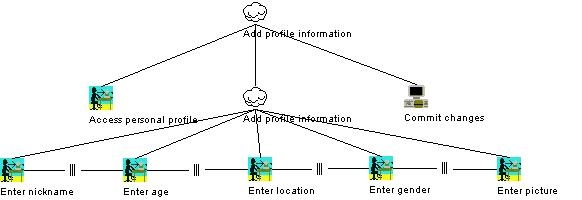
\includegraphics[width=\textwidth]{CTT_Add.png}
 \captionof{figure}[Add personal profile CTT]{CTT to add information on the personal profile.}
\end{minipage}
$\;$ \\ \\
%----------------------------------------------------------------------------------------------------------
\underline{Requirement:} ``The registered users should be able to delete any information on their personal profile.'' \\ \\
\underline{Task:} Delete information on the personal profile. \\
When a user wants to delete any information of their personal profile, he or she should first navigate to the profile information, delete the desired information and save the deletions made. \\ \\
\underline{Decomposition:}
\begin{itemize}
\item Access the personal profile.
\item Delete the nickname.
\item Delete the age.
\item Delete the location.
\item Delete the gender.
\item Delete the picture.
\item Commit the changes. 
\end{itemize}
\noindent\begin{minipage}{\textwidth}
    \centering
   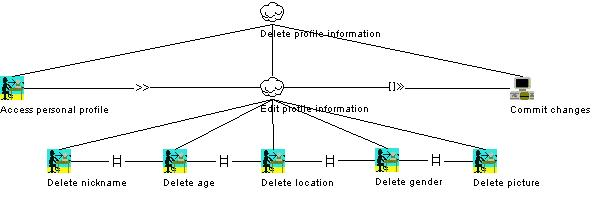
\includegraphics[width=\textwidth]{CTT_Profile_Delete.png}
 \captionof{figure}[Delete personal profile CTT]{CTT to delete information on the personal profile.}
\end{minipage}
$\;$ \\ \\
%----------------------------------------------------------------------------------------------------------
\underline{Requirement:} ``The users should be able to search for other users, based on the profile information.'' \\ \\
\underline{Task:} Search for other members, based on their profile information. \\
A user must be able to search for other members, based on the username / nickname, age, gender, range or location. \\ \\
\underline{Decomposition:}
\begin{itemize}
\item Enter the username.
\item Enter the age.
\item Enter the gender.
\item Enter the range.
\item Enter the location.
\item Display the results.
\end{itemize}
\noindent\begin{minipage}{\textwidth}
    \centering
   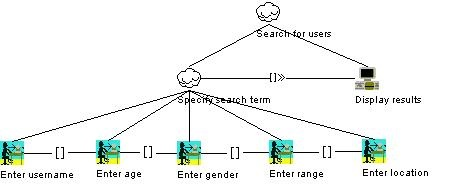
\includegraphics{CTT_Search_Profile.png}
 \captionof{figure}[Search personal profile CTT]{CTT to search for other users, based on the profile information.}
\end{minipage}
$\;$ \\ \\
%----------------------------------------------------------------------------------------------------------
\underline{Requirement:} ``The user profiles of other members can be seen by the users.'' \\ \\
\underline{Task:} Browse the user profiles of other members. \\
Each registered user can browse and see the profile of any other registered user. To do so, a user accesses the browsing function and the system displays an alphabetic list of users.\\ \\
\underline{Decomposition:}
\begin{itemize}
\item Access the browsing function.
\item Display an alphabetic list.
\end{itemize}
\noindent\begin{minipage}{\textwidth}
    \centering
   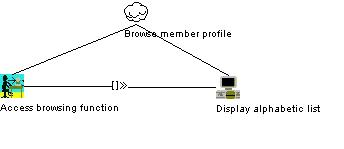
\includegraphics{CTT_Member_Profile.png}
 \captionof{figure}[Browse member profile CTT]{CTT to browse (through) other member's profiles. This implies they (the profiles) can be seen by the users.}
\end{minipage}
$\;$ \\ \\
%----------------------------------------------------------------------------------------------------------
\underline{Requirement:} ``The users should be able to put messages on any user's wall.'' \\ \\
\underline{Task:} Put messages on a user's wall. \\
Each registered user can put messages on the personal wall of any other registered user. Therefore, a user navigates to the wall of the desired user, writes the message in a destined box and saves the changes. Next, the message is made visible on the profile.\\ \\
\underline{Decomposition:}
\begin{itemize}
\item Navigate to the user wall of the desired user.
\item Enter the message (write the message).
\item Save changes and make the message visible to others.
\end{itemize}
\noindent\begin{minipage}{\textwidth}
    \centering
   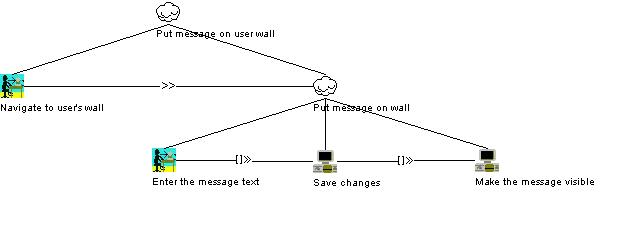
\includegraphics[width=\textwidth]{CTT_Put_Message.png}
 \captionof{figure}[Put message on user wall CTT]{CTT to put a message on the wall of a user.}
\end{minipage}
$\;$ \\ \\
%----------------------------------------------------------------------------------------------------------
\underline{Requirement:} ``The users should be able to answer to a message on their own wall.'' \\ \\
\underline{Task:} Answer to a message on their own wall. \\
Each registered user is able to answer to a message that has been put before on their personal profile wall. Therefore, a user navigates to their own wall, selects the desired message, writes the answer to a message in a therefore destined box and saves the changes. Next, the answer (the message) is made visible on the profile.\\ \\
\underline{Decomposition:}
\begin{itemize}
\item Navigate to the personal user wall.
\item Select the desired message.
\item Enter the answer to a message.
\item Save changes and make the answer visible to others.
\end{itemize}
\noindent\begin{minipage}{\textwidth}
    \centering
   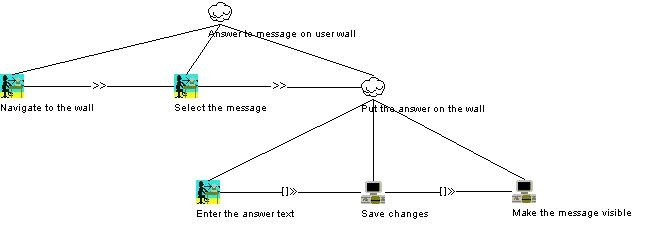
\includegraphics[width=\textwidth]{CTT_Answer_Message.png}
 \captionof{figure}[Answer message on user wall CTT]{CTT to answer to a message already posted on the user's wall.}
\end{minipage}
$\;$ \\ \\
%----------------------------------------------------------------------------------------------------------
\underline{Requirement:} ``The users should be able to delete a message from their personal wall.'' \\ \\
\underline{Task:} Delete a message from their personal wall. \\
In order to delete a message from the personal wall, the user navigates to their personal wall, selects the message and after the confirmation the message is actually deleted. \\ \\ 
\underline{Decomposition:}
\begin{itemize}
\item Navigate to the personal user wall.
\item Select the desired message.
\item The system asks for confirmation.
\item The user confirms the deletion.
\item The message gets actually deleted.
\end{itemize}
\noindent\begin{minipage}{\textwidth}
    \centering
   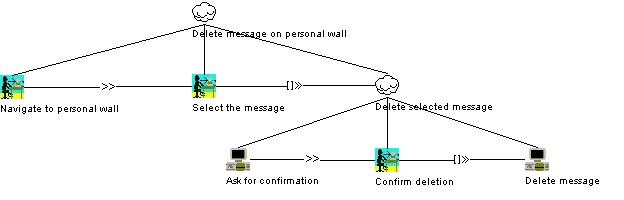
\includegraphics[width=\textwidth]{CTT_Delete_Message.png}
 \captionof{figure}[Delete message on user wall CTT]{CTT to delete to a message from the user's wall.}
\end{minipage}
$\;$ \\ \\
%----------------------------------------------------------------------------------------------------------
\underline{Requirement:} ``The users should be able to communicate to other registered users by sending them private messages.'' \\ \\
\underline{Task:} Send a private message to a registered user. \\
To sent a message to a registered user, a user navigates to the profile (possibly after performing a search) of the user he wishes to send a message to and clicks on a link to send the private message. After typing the message text, the user confirms the sending of the message.\\ \\
\underline{Decomposition:}
\begin{itemize}
\item Search for the user (optional).
\item Navigate to its user profile.
\item Click on a link to send the message.
\item Type the message text.
\item Confirm sending the message.
\end{itemize}
\noindent\begin{minipage}{\textwidth}
    \centering
   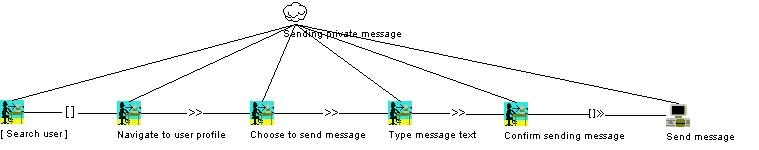
\includegraphics[width=\textwidth]{CTT_Send_PM.png}
 \captionof{figure}[Send private message CTT]{CTT to sent a private message to a registered user.}
\end{minipage}
$\;$ \\ \\
%----------------------------------------------------------------------------------------------------------
\underline{Requirement:} ``The users should be able to `like' other users.'' \\ \\
\underline{Task:} ``Like'' another user. \\
To ``like'' another user, a registered user navigates to its user profile, possibly after performing a search to find the user he or she wishes to like. The user clicks on a ``like'' button and the like is registered. \\ \\
\underline{Decomposition:}
\begin{itemize}
\item Search for the user (optional).
\item Navigate to its user profile.
\item Click on a ``like'' button.
\item The ``like'' is registered.
\end{itemize}
\noindent\begin{minipage}{\textwidth}
    \centering
   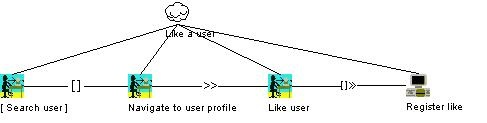
\includegraphics[width=\textwidth]{CTT_Like.png}
 \captionof{figure}[Like user CTT]{CTT to like another user.}
\end{minipage}
$\;$ \\ \\
%----------------------------------------------------------------------------------------------------------
\underline{Requirement:} ``The users should be able to manage their `liked' list.'' \\ \\
\underline{Task:} Manage their personal `liked' list. \\
Each time a user likes another user, this user is added to their ``liked'' list. To manage this list, a user is able to remove (VOORLOPIG ALLEEN REMOVE) users from the list. \\ \\
\underline{Decomposition:}
\begin{itemize}
\item Navigate to the ``liked'' list.
\item Select the desired user.
\item Choose to remove the user from the list.
\item Ask for confirmation.
\item Confirm the deletion of the user from the list.
\item Remove the user.
\end{itemize}
\noindent\begin{minipage}{\textwidth}
    \centering
   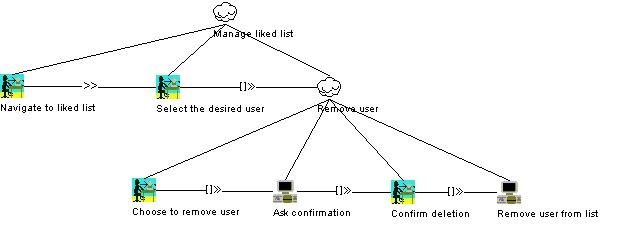
\includegraphics[width=\textwidth]{CTT_LikeList.png}
 \captionof{figure}[Manage liked list CTT]{CTT to manage the personal liked list.}
\end{minipage}
$\;$ \\ \\
%----------------------------------------------------------------------------------------------------------
\underline{Requirement:} ``The user should be notified in case of profile updates of their `liked' users.'' \\ \\
\underline{Task:} Notify a user in case of profile updates. \\
Each time a ``liked'' user on the ``liked'' list updates its profile, a notification to the user is sent as a pop-up message and sound.\\ \\
\underline{Decomposition:}
\begin{itemize}
\item Monitor profile updates.
\item If profile is updated:
\begin{itemize}
\item Show notification message.
\item Play sound.
\end{itemize}
\end{itemize}
\noindent\begin{minipage}{\textwidth}
    \centering
   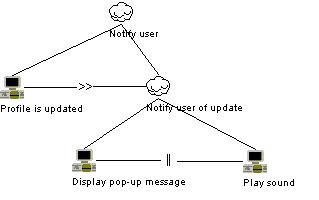
\includegraphics[scale=1.2]{CTT_Notify.png}
 \captionof{figure}[Notify user CTT]{CTT to notify a user by means of a pop-up message and sound when the profile of a user on their liked list changes.}
\end{minipage}
$\;$ \\ \\
%----------------------------------------------------------------------------------------------------------
\underline{Requirement:} ``The users should be able to send another user an attention. These attentions should be the following:
\begin{itemize}
\item A bouquet of flowers
\item A handshake
\item A Smiley
\item A kiss
\item A tap on the back	
\item A thumbs up	
\item A bottle of wine''
\end{itemize}
\underline{Task:} Send an attention. \\
An attention can be send to a user in the form of a bouquet of flowers, a handshake, a smiley, a kiss, a tap on the back, a thumbs up or a bottle of wine. To do so, a user navigates to the user's profile of whom he or she wants to send the attention to (possibly after a search) and chooses which kind of attention he or she wants to send. \\ \\
\underline{Decomposition:}
\begin{itemize}
\item Search for a user's profile (optional).
\item Navigate to the user's profile.
\item Choose to send an attention.
\item Choose the desired attention.
\item Confirm.
\end{itemize}
\noindent\begin{minipage}{\textwidth}
    \centering
   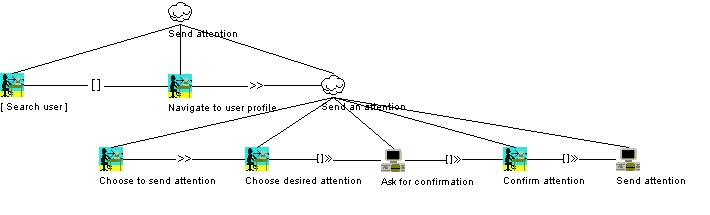
\includegraphics[width=\textwidth]{CTT_Attention.png}
 \captionof{figure}[Send attention CTT]{CTT to send an attention to a desired user.}
\end{minipage}
$\;$ \\ \\
%----------------------------------------------------------------------------------------------------------
\underline{Requirement:} ``The users should be informed about a received attention and should be able to return the favor.'' \\ \\
\underline{Task:} Inform user about a received attention. \\
In case of a user sending an attention to another user, the user should be notified by a pop-up screen where the user can directly return the favor or just ignore it. \\ \\
\underline{Decomposition:}
\begin{itemize}
\item Attention has been sent.
\item User receives the attention.
\item Show a pop-up screen.
\item Ignore the attention or reply to it.
\item In case of replying to it, choose the attention and send it.
\end{itemize}
\noindent\begin{minipage}{\textwidth}
    \centering
   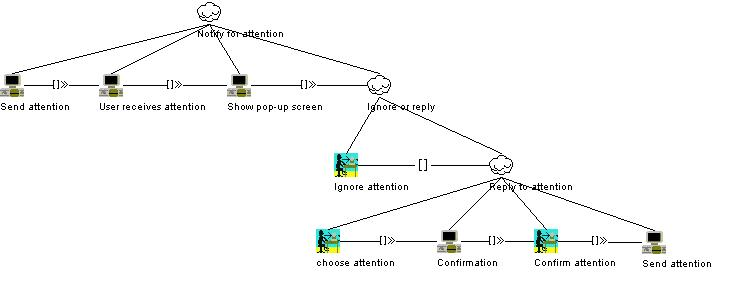
\includegraphics[width=\textwidth]{CTT_AttentionNotify.png}
 \captionof{figure}[Notify for attention CTT]{CTT to notify when an attention has been sent to the user.}
\end{minipage}
$\;$ \\ \\
%----------------------------------------------------------------------------------------------------------
\underline{Requirement:} ``The users should be able to message with randomly selected users, based on the selected gender and age.'' \\ \\
\underline{Task:} Send message to any user, based on gender and age. \\
After searching for age and gender, a matched result list is displayed from where the user can select people to message with. So the user fills in the age and gender, the system displays a list based on the age and gender. The user selects a person and a chatbox is opened. \\ \\
\underline{Decomposition:}
\begin{itemize}
\item Search for age and gender.
\item Display the result list.
\item Select the desired person.
\item Send message to person.
\end{itemize}
\noindent\begin{minipage}{\textwidth}
    \centering
   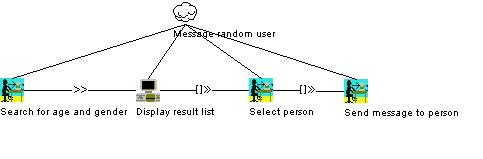
\includegraphics[width=\textwidth]{CTT_Message_Random.png}
 \captionof{figure}[Send message to any user CTT]{CTT to send a message to a user basd on age and gender.}
\end{minipage}
$\;$ \\ \\
%----------------------------------------------------------------------------------------------------------
\underline{Requirement:} ``The users should be able to block and report other users.'' \\ \\
\underline{Task:} Block and report a user. (EN SEND MESSAGE TO ADMINISTRATOR?????) TBD\ldots \\
\underline{Decomposition:}
\begin{itemize}
\item Block user.
\item Report user.
\end{itemize}
\noindent\begin{minipage}{\textwidth}
    \centering
   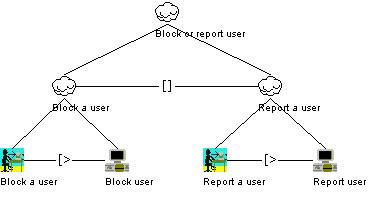
\includegraphics{CTT_Block.png}
 \captionof{figure}[Block user CTT]{CTT to block or report a user.}
\end{minipage}
$\;$ \\ \\
%----------------------------------------------------------------------------------------------------------
\underline{Requirement:} ``The users should be able to log off.'' \\ \\
\underline{Task:} Log off. \\
The user is logged off and is redirected to the home page. \\ \\
\underline{Decomposition:}
\begin{itemize}
\item Log off.
\item Redirect to the home page.
\end{itemize}
\noindent\begin{minipage}{\textwidth}
    \centering
   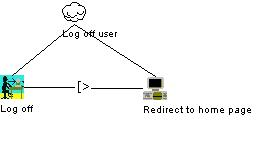
\includegraphics{CTT_Logoff.png}
 \captionof{figure}[Log off user CTT]{CTT to log off a user.}
\end{minipage}
$\;$ \\ \\
%----------------------------------------------------------------------------------------------------------
\underline{Requirement:} ``The users should be able to terminate their account.'' \\ \\
\underline{Task:} Terminate account. \\ \\
\begin{itemize}
\item Terminate account.
\item Redirect to the home page.
\end{itemize}
\noindent\begin{minipage}{\textwidth}
    \centering
   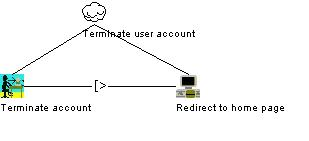
\includegraphics{CTT_Terminate.png}
 \captionof{figure}[Terminate account CTT]{CTT to terminate a user account.}
\end{minipage}
$\;$ \\ \\
%----------------------------------------------------------------------------------------------------------
\underline{Requirement:} ``Detailed personal information.'' \\ \\
\underline{Task:} Provide detailed personal information on the user profile \\
When a user navigates to its user profile, allow to give detailed personal information consisting of their username / nickname, age, gender, location and picture. \\ \\
\underline{Decomposition:}
\begin{itemize}
\item Navigate to user profile.
\item Display nickname.
\item Display age.
\item Display location.
\item Display gender.
\item Display picture.
\end{itemize}
\noindent\begin{minipage}{\textwidth}
    \centering
   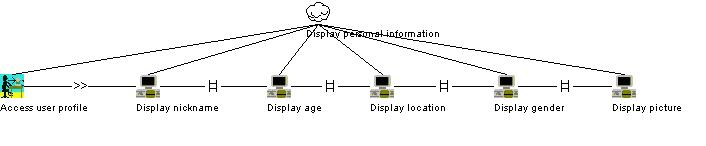
\includegraphics[width=\textwidth]{CTT_Personal.png}
 \captionof{figure}[Personal information CTT]{CTT to display the detailed personal information of a user.}
\end{minipage}
$\;$ \\ \\
%----------------------------------------------------------------------------------------------------------
\underline{Requirement:} ``Detailed information about other users' profiles.'' \\ \\
\underline{Task:} Provide detailed information about the profile of other users. \\
When a user navigates to the user profile of any registered user, allow to give detailed personal information consisting of their username / nickname, age, gender, location and picture. \\ \\
\underline{Decomposition:}
\begin{itemize}
\item Navigate to foreign user profile.
\item Display nickname.
\item Display age.
\item Display location.
\item Display gender.
\item Display picture.
\end{itemize}
\noindent\begin{minipage}{\textwidth}
    \centering
   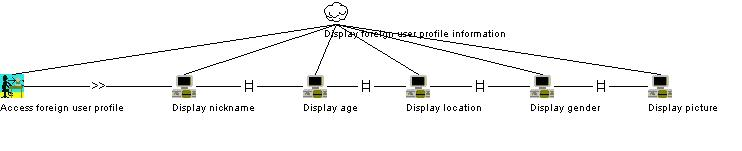
\includegraphics[width=\textwidth]{CTT_Foreign.png}
 \captionof{figure}[Foreign user information CTT]{CTT to display the detailed personal information of a foreign user.}
\end{minipage}
%----------------------------------------------------------------------------------------------------------
\subsection{Audience class Administrators}
%----------------------------------------------------------------------------------------------------------
\underline{Requirement:} ``The administrators should be able to browse through all user profiles.'' \\ \\
\underline{Task:} Browse through all user profiles. \\ \\
\underline{Decomposition:}
\begin{itemize}
\item Access browsing function.
\item List profiles.
\item Browse profiles.
\end{itemize}
\noindent\begin{minipage}{\textwidth}
    \centering
   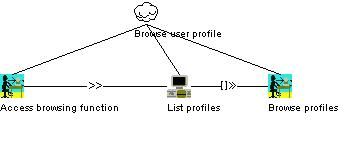
\includegraphics{CTT_Browse.png}
 \captionof{figure}[Browse profiles CTT]{CTT to browse any user profile.}
\end{minipage}
$\;$ \\ \\
%----------------------------------------------------------------------------------------------------------
\underline{Requirement:} ``The administrator should receive a message when another user blocks or reports a user.'' \\ \\
\underline{Task:} Receive a message when a user is blocked. \\
Upon blocking a user, the administrator receives a message.
\underline{Decomposition:}
\begin{itemize}
\item User blocks another user.
\item Administrator receives message.
\end{itemize}
\noindent\begin{minipage}{\textwidth}
    \centering
   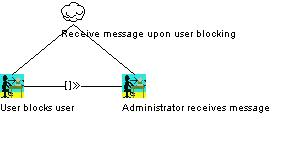
\includegraphics{CTT_Admin_Message.png}
 \captionof{figure}[User blocking message CTT]{CTT to send a message to the administrator when a user blocks another user.}
\end{minipage}
$\;$ \\ \\
%----------------------------------------------------------------------------------------------------------
\underline{Requirement:} ``The administrator can send a message to any other user.'' \\ \\
\underline{Task:} Send message to user. \\
The administrator searches for the desired user or accesses the browsing function directly to retrieve the list of users. A user is selected, the message is typed and sent.
\underline{Decomposition:}
\begin{itemize}
\item Search for the desired user (optional).
\item Access the browsing function.
\item Display alphabetical list of users.
\item Select the desired user.
\item Type the message text.
\item Send the message.
\end{itemize}
\noindent\begin{minipage}{\textwidth}
    \centering
   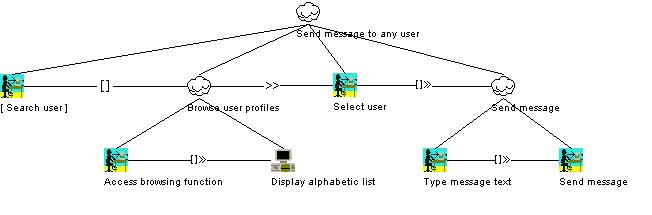
\includegraphics[width=\textwidth]{CTT_Admin_Send_Message.png}
 \captionof{figure}[Send message to any user CTT]{CTT to send a message to any user.}
\end{minipage}
$\;$ \\ \\
%----------------------------------------------------------------------------------------------------------
\underline{Requirement:} ``The administrator can block, disable or delete any user account.'' \\ \\
\underline{Task:} Block, disable or delete user account. \\
The administrator has the choice to block, disable or delete a user account. For each choice, it is possible to either search a user or browse the user profiles. Then the desired user has to be selected and respectively blocked, disabled or deleted. \\ \\
\underline{Decomposition:}
\begin{itemize}
\item Choose between block, disable or delete  a user account.
\item In case of blocking a user account:
\begin{itemize}
\item Search for a user account.
\item Or browse the user profile list.
\item Select the desired user.
\item Block the user.
\end{itemize}
\item In case of disabling a user account:
\begin{itemize}
\item Search for a user account.
\item Or browse the user profile list.
\item Select the desired user.
\item Disable the user.
\end{itemize}
\item In case of deleting a user account:
\begin{itemize}
\item Search for a user account.
\item Or browse the user profile list.
\item Select the desired user.
\item Delete the user.
\end{itemize}
\end{itemize}
\noindent\begin{minipage}{\textwidth}
    \centering
   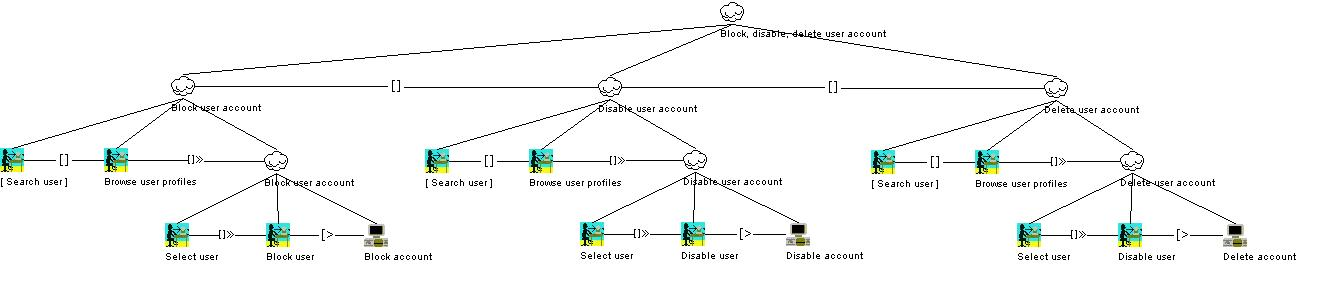
\includegraphics[angle=270,scale=0.5]{CTT_Admin_Block_Disable_Delete.png}
 \captionof{figure}[Send message to any user CTT]{CTT to send a message to any user.}
\end{minipage}
%----------------------------------------------------------------------------------------------------------


\section{Information modeling}

In the information modeling phase, the domain model as UML diagrams is created. This has been done by using the WebRatio tool. The result is depicted in the figure below:
$\;$ \\ \\
\noindent\begin{minipage}{\textwidth}
    \centering
   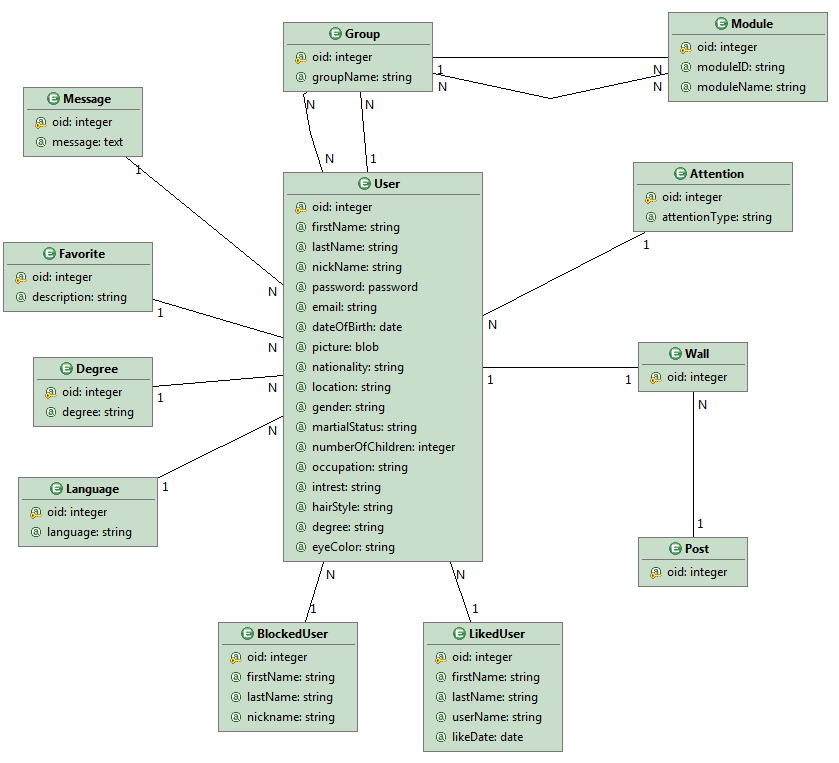
\includegraphics[scale=0.8]{DomainModel.png}
 \captionof{figure}[Domain model]{Domain model created using WebRatio.}
\end{minipage}


\clearpage

\section{Navigational modeling}

In the navigational modeling phase, the structure of the website is modeled. First, we will start with the conceptual structual model, providing a general overview of the website's navigation structure, called tracks. Then, each individual track is worked out in more detail. \\
The figures have been created using Microsoft Office Visio 2010. To be more specific, the shapes of the ``Data Flow Diagram'' type have been used. The graphics are exported as vector images and thus feature an infinite resolution.

\subsection{Conceptual Structural Model}

The figure below illustrates the conceptual structure of the web application. As previously mentioned in section \ref{sec:visitorclass}, the visitor audience class is the most general class with the least privileges, followed by the registered users. There exist two types of registered users, each with specific requirements and thus two seperate tracks.
$\;$ \\ \\
\noindent\begin{minipage}{\textwidth}
    \centering
   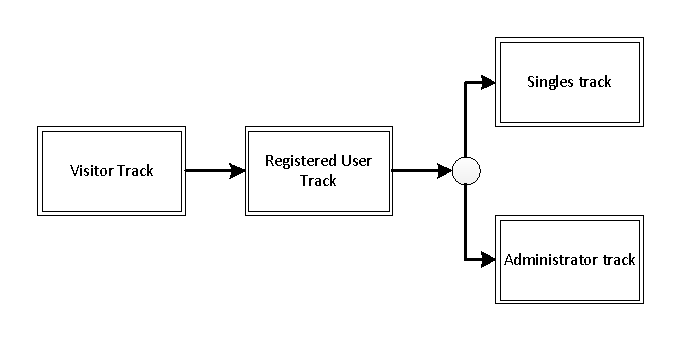
\includegraphics[scale=1.3]{Nav_Concept.pdf}
 \captionof{figure}[Conceptual structural model]{Conceptual structural model of the web application.}
\end{minipage}


\subsection{Visitor navigational track}

The visitor track is the most general track. Visitors are able to search for members, that is, the so-called ``singles'' audience class, to register a new user account and to login. Additionally, information about the 10 last logged in members is shown.
$\;$ \\ \\
\noindent\begin{minipage}{\textwidth}
    \centering
   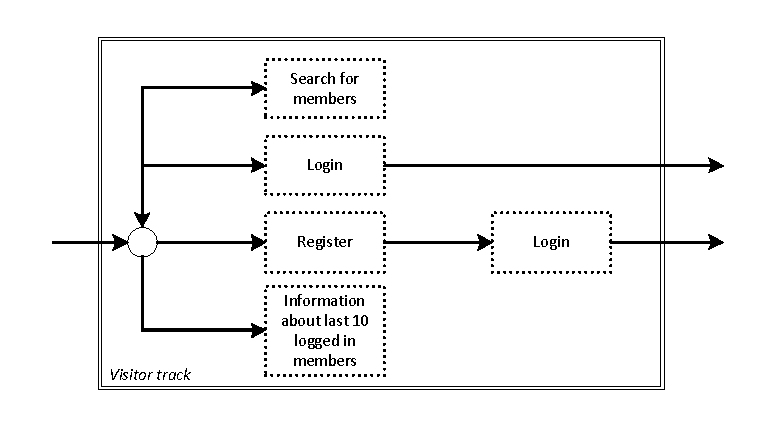
\includegraphics[scale=1.3]{Nav_Visitor_Track.pdf}
 \captionof{figure}[Visitor track]{Visitor navigational track.}
\end{minipage}
$\;$ \\ 

\subsection{Registered user navigational track}

The registered users - both administrators and singles, have more functionality than visitors. For example, they are able to edit their profile, search for users, logout and terminate their account. The complete functionality is depicted in the figure below.
$\;$ \\
\noindent\begin{minipage}{\textwidth}
    \centering
   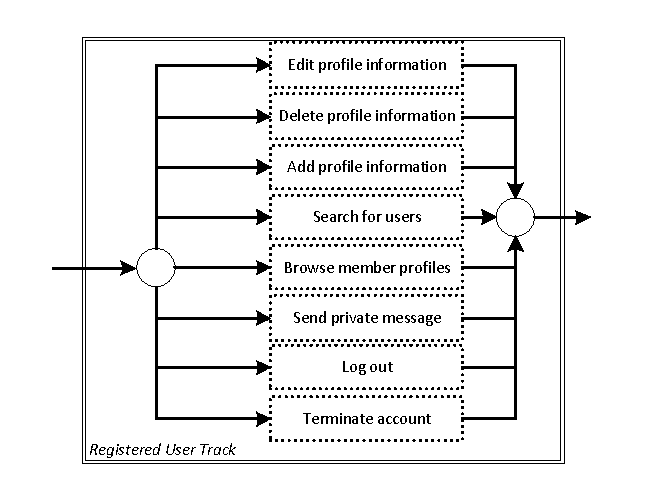
\includegraphics[scale=1]{Nav_RegisteredUser_Track.pdf}
 \captionof{figure}[Registered User track]{Registered User navigational track.}
\end{minipage}
$\;$ \\ 

\subsection{Singles navigational track}

As previously mentioned in section \ref{sec:singlesclass}, the ``singles'' audience class is the actual target audience of the web application. They have all the functionality and privileges of the ``registered users'' audience class and in addition, very much more functionality is availabe. For example, they can put messages on another user's wall, delete messages on their own wall, like users, and so on\ldots.\\
For a complete overview of the requirements, the reader is invited to take a look at the figure below, that depicts the singles track; that is, the navigational flow of the ``singles'' audience class.
$\;$ \\
\noindent\begin{minipage}{\textwidth}
    \centering
   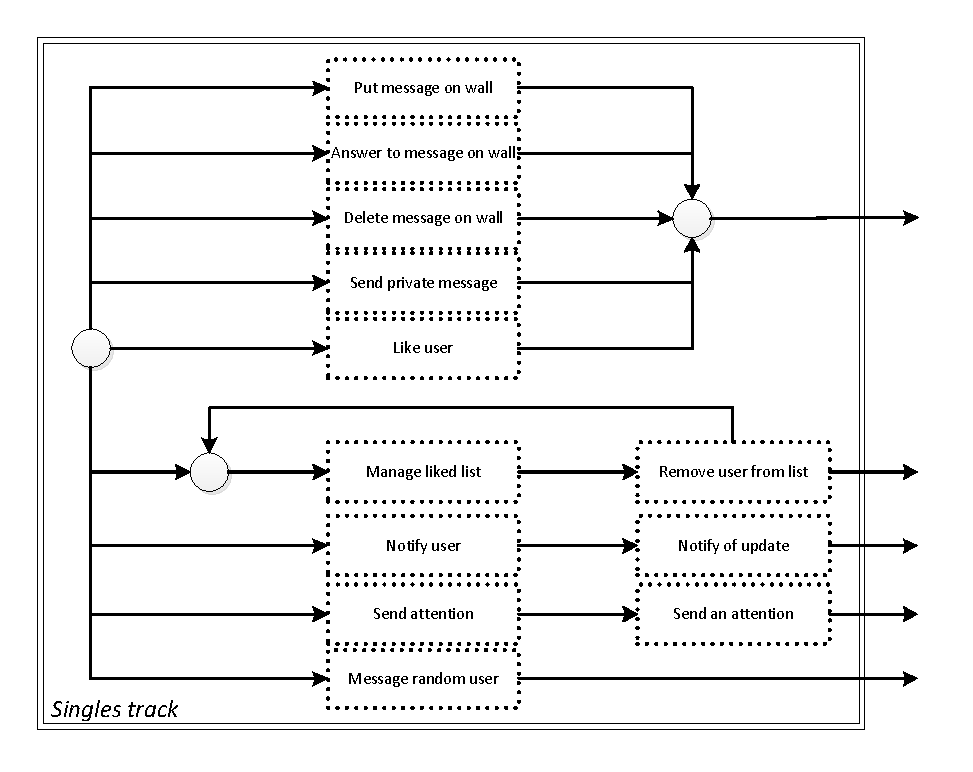
\includegraphics[scale=1]{Nav_Singles_Track.pdf}
 \captionof{figure}[Singles track]{Singles navigational track.}
\end{minipage}
$\;$ \\ 

\subsection{Administrator navigational track}

The ``administrator'' audience class is a subclass of the ``registered users'' class. The have the same privileges as them, but can browse all user profiles, send a message to any user, as well as deleting any user account.

$\;$ \\
\noindent\begin{minipage}{\textwidth}
    \centering
   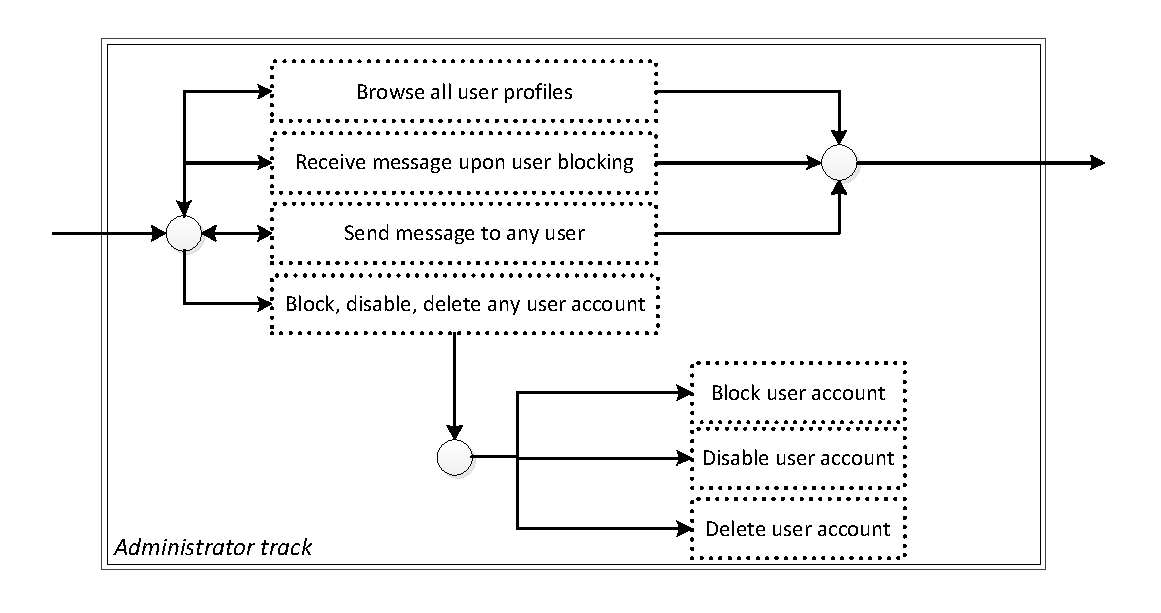
\includegraphics[scale=0.8]{Nav_Administrator_Track.pdf}
 \captionof{figure}[Administrator track]{Administrator navigational track.}
\end{minipage}
$\;$ \\ \\
The upcoming sections describe the \textbf{fully specified task navigational models}. For each dotted square component in the different tracks, a task navigational model is made. These correspond with the CTT's. They are also made with Visio 2010 and are exported as svg image.

\subsection{Login}

When a visitor wants to login, he or she specifies his or her credentials which contain of a username and a password. The visitor submits the form, is authenticated and redirected.

$\;$ \\
\noindent\begin{minipage}{\textwidth}
    \centering
   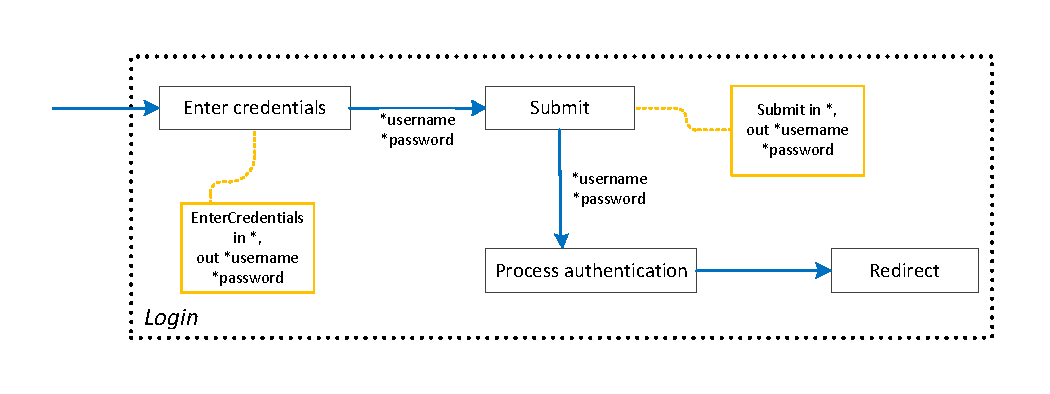
\includegraphics[scale=0.9]{Nav_Login.pdf}
 \captionof{figure}[Login WSDM model]{Login task navigational model.}
\end{minipage}
$\;$ \\ 

\subsection{Register new user}

The task navigational model for registering a new user is depicted in the figure below. The visitor enters the necessary credentials (see figure for a complete list) and its account is registered. Upon registration, the user - registered user now - is logged in immediately and redirected to its profile page - as indicated in the login navigational model.
$\;$ \\
\noindent\begin{minipage}{\textwidth}
    \centering
   \includegraphics[scale=1]{Nav_Register.pdf}
 \captionof{figure}[Register user WSDM model]{Register new user task navigational model.}
\end{minipage}

\subsection{Search for members}

A visitor can also search for members. To do so, the visitor enters the nickname, age, location and gender - none of them is obligatory, see the IFML site structure design diagrams - and the system processes the data and shows the top 10 results.

$\;$ \\
\noindent\begin{minipage}{\textwidth}
    \centering
   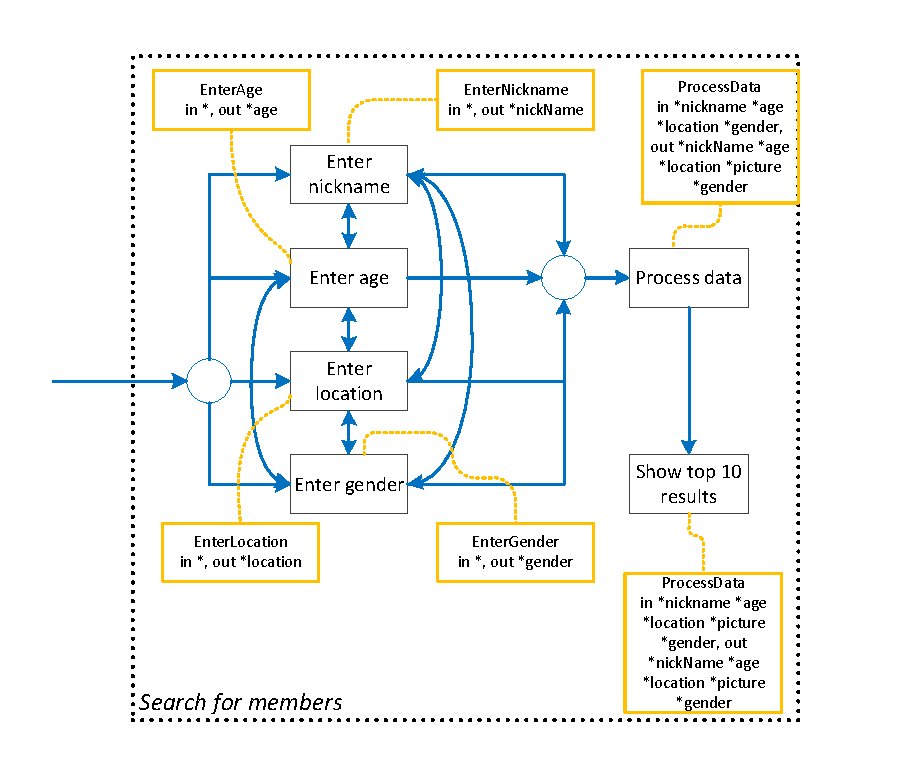
\includegraphics[scale=1]{Nav_SearchForMembers.pdf}
 \captionof{figure}[Search for members WSDM model]{Search for members task navigational model.}
\end{minipage}

\subsection{Information about the 10 last logged in members}

By default, the information about the 10 last logged in members is shown. The data is delivered by the system and displayed.

$\;$ \\
\noindent\begin{minipage}{\textwidth}
    \centering
   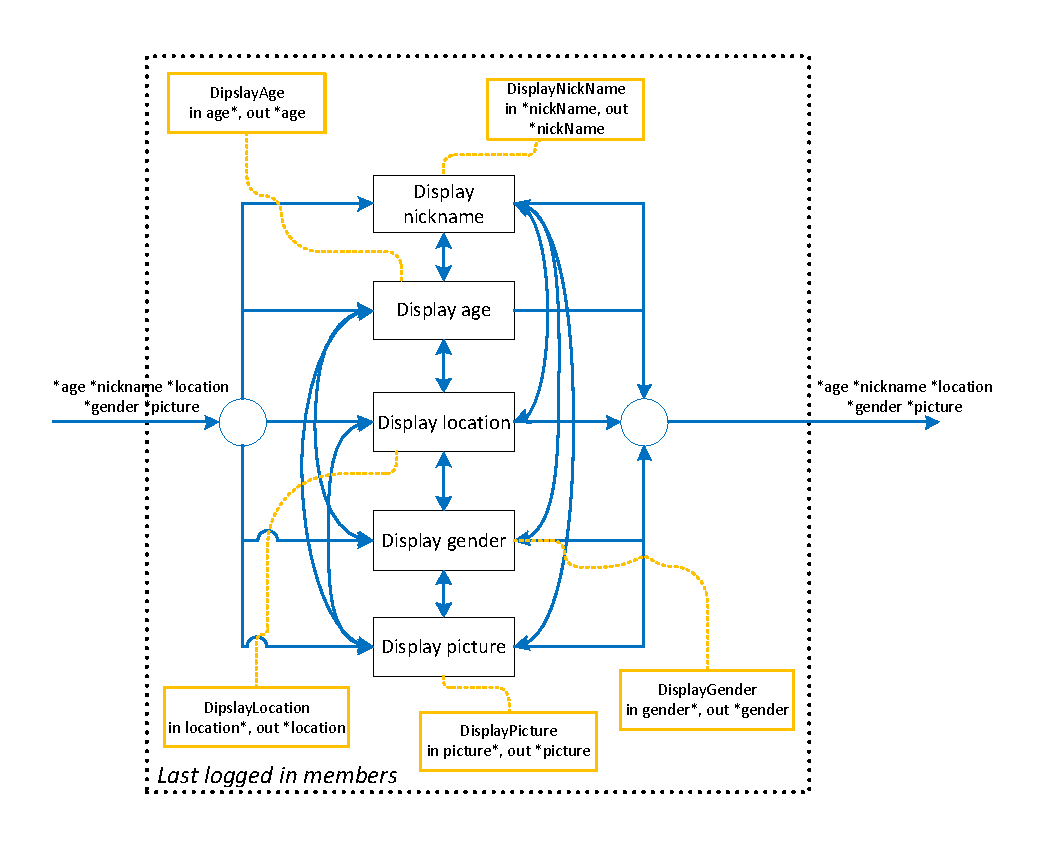
\includegraphics[scale=1]{Nav_LastLoggedInMembers.pdf}
 \captionof{figure}[10 last logged in members WSDM model]{The 10 last logged in members navigational model.}
\end{minipage}

\clearpage

\subsection{Change, add and delete profile information}

The first step in changing / editing the personal profile of any registered user is accessing the profile. Then the user is able to change the nickname, age, location, gender and picture. All the information is passed to the system. \\
Deleting profile information - i.e., leaving blank some input form fields uses the same navigational model and is therefore not drawn again. \\
Adding profile information - i.e., filling in input form fields uses also the same navigational model and is again thus not drawn again.
$\;$ \\
\noindent\begin{minipage}{\textwidth}
    \centering
   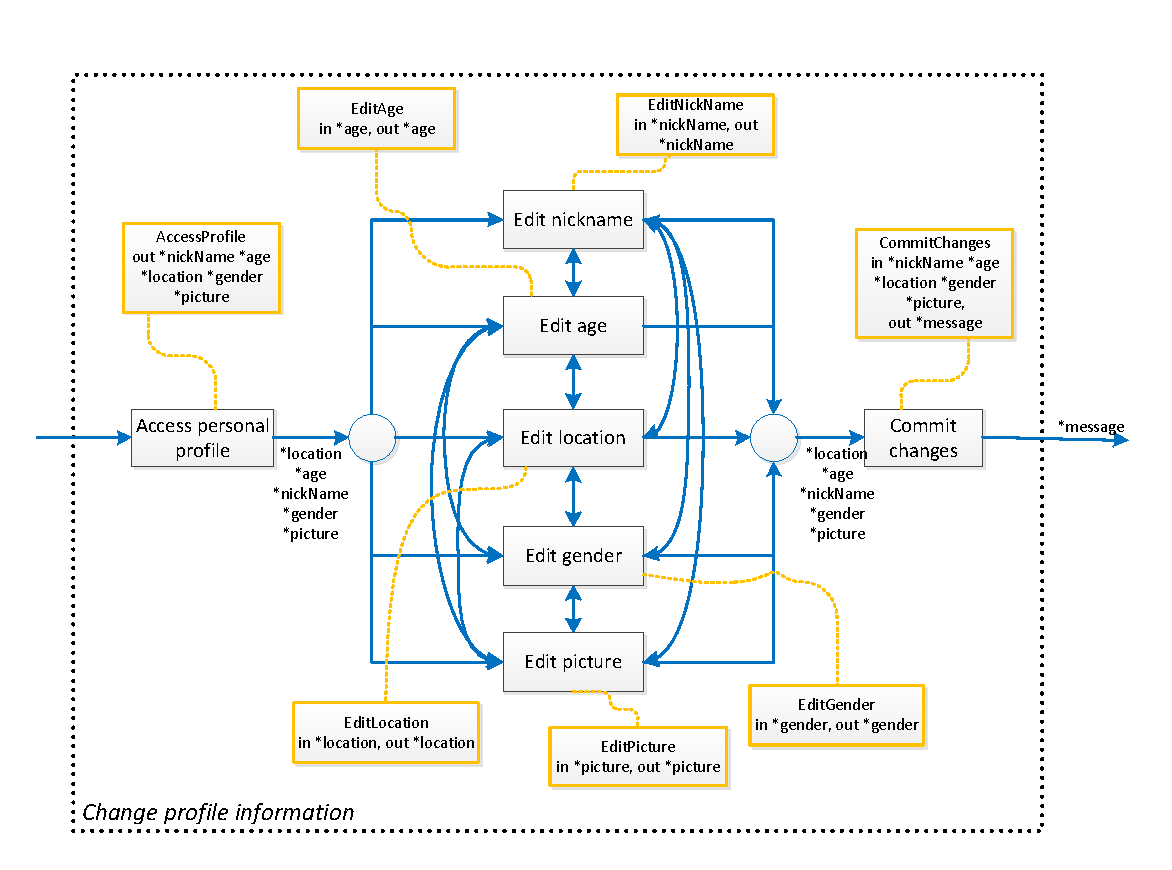
\includegraphics[scale=0.85]{Nav_ChangeProfileInformation.pdf}
 \captionof{figure}[Change, (add en delete) profile information WSDM model]{Change (,add en delete) profile information navigational model.}
\end{minipage}

\subsection{Search for users}

Registered users are able to search for users. To do so, the search criteria are provided to the system. These are: nickname, age, location, gender and range. Subsequently, the system displays the results. Note that none of the search criteria are required. If no criteria are supplied to the system, all users are returned.
$\;$ \\
\noindent\begin{minipage}{\textwidth}
    \centering
   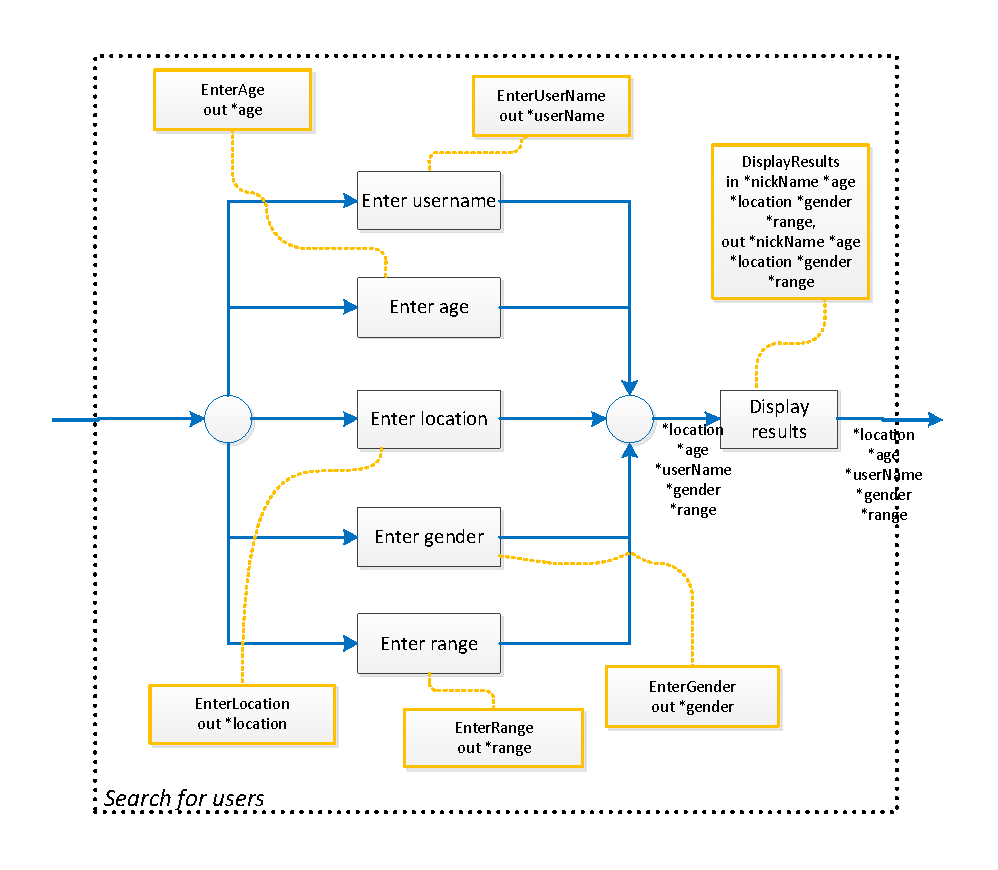
\includegraphics[scale=1]{nav_SearchUsers.pdf}
 \captionof{figure}[Search users WSDM model]{Search for users navigational model.}
\end{minipage}

\subsection{Browse user profiles}

Registered users are able to browse each other's user profiles. The figure below depicts this navigational model. The figure is quite straightforward and does not require more information to be specified.
$\;$ \\
\noindent\begin{minipage}{\textwidth}
    \centering
   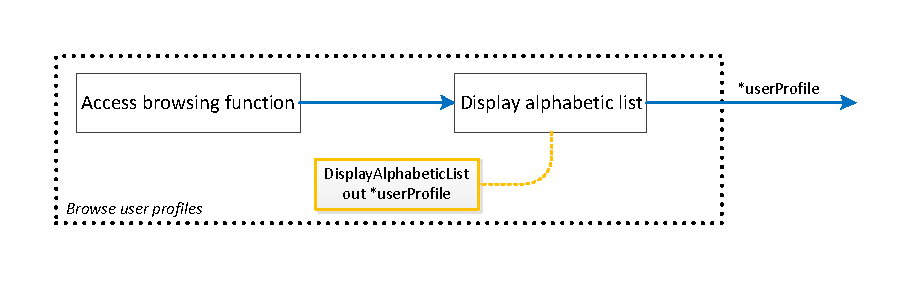
\includegraphics[scale=1]{nav_BrowseUserProfile.pdf}
 \captionof{figure}[Browse user profiles WSDM model]{Browse user profiles navigational model.}
\end{minipage}

\subsection{Put message on user wall}

Any registered user - whether it is a ``single'' or ``administrator'', can put a message on a ``single'' ' wall. To do so, the user navigates to the user's wall, chooses to place a message on its wall and enters the message text. The system makes the text visible to the rest. \\
The profileID is also supplied to identify the user's wall. The time is provided to the system as well to be able to know the date the message has been posted.

$\;$ \\
\noindent\begin{minipage}{\textwidth}
    \centering
   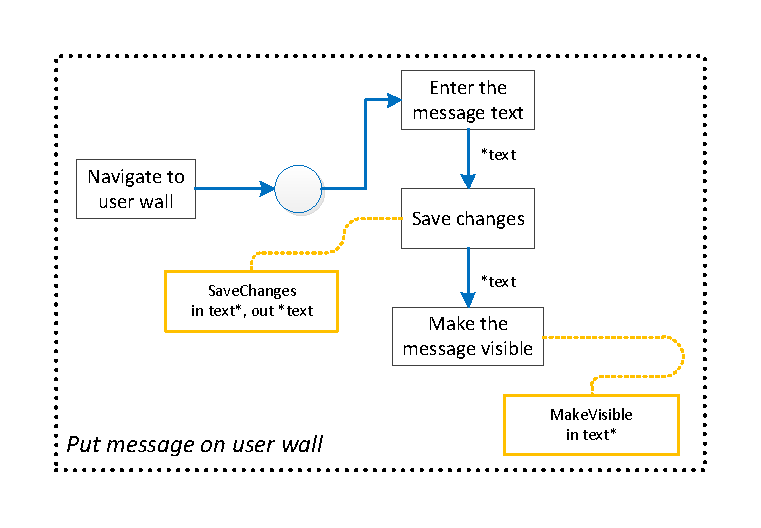
\includegraphics[scale=1]{nav_PutMessageOnUserWall.pdf}
 \captionof{figure}[Put message on user wall]{Put message on user wall.}
\end{minipage}

\subsection{Answer to a message on personal wall}

Once the message has been posted on the user's wall, the ``single'' can reply to the posted message. To do so, the user navigates to its personal wall, selects the message, enters a text and posts the answer. The system save the new reply. During the entire process, the unique ID of the message is passed through the system. 

$\;$ \\
\noindent\begin{minipage}{\textwidth}
    \centering
   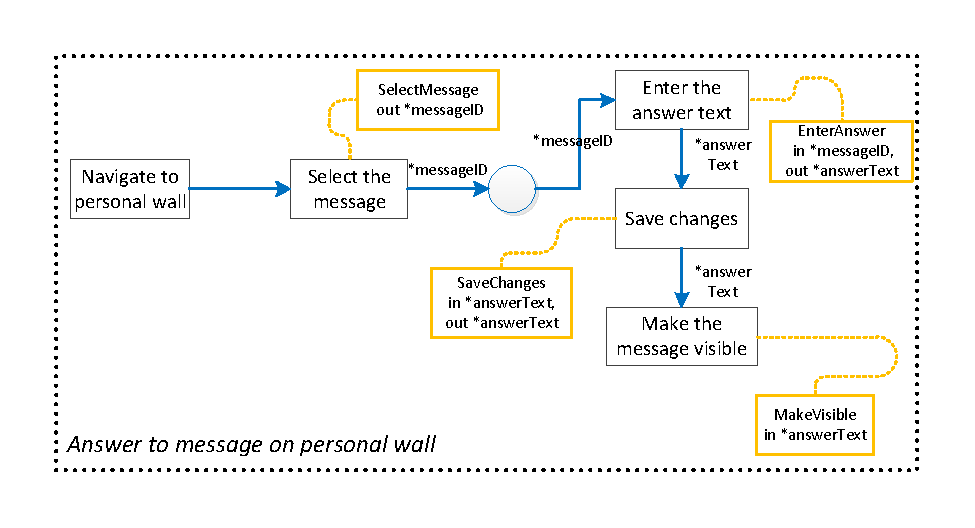
\includegraphics[scale=1]{nav_AnswerMessagePersonalWall.pdf}
 \captionof{figure}[Answer message on user wall]{Answer message on personal wall.}
\end{minipage}

\subsection{Delete message on personal wall}

Deletion of a message follows roughly the same procedure as answering to a message on the personal wall. Instead of answering to a message, the system now asks for confirmation. The ``single'' confirms or rejects the deletion. When rejected, he is returned to the personal wall again. In case of confirmation, the message is deleted.
$\;$ \\
\noindent\begin{minipage}{\textwidth}
    \centering
   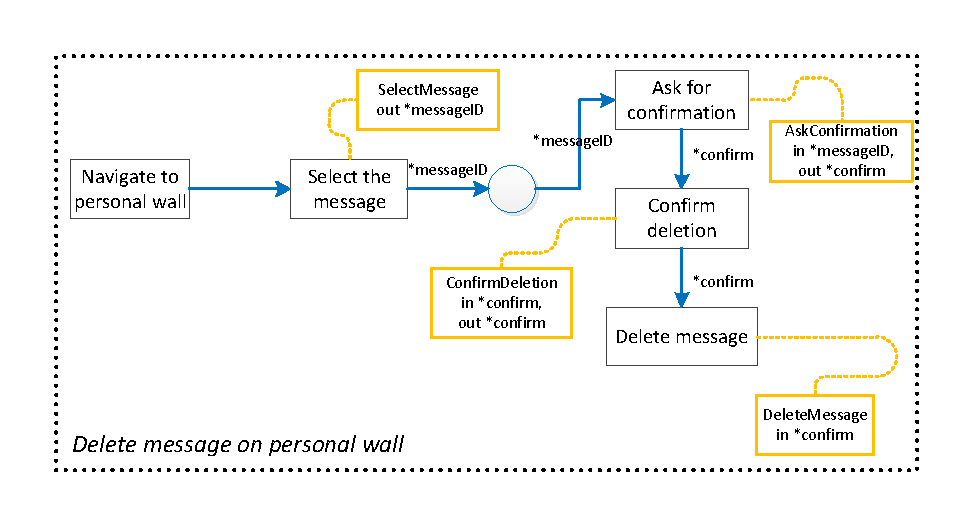
\includegraphics[scale=1]{nav_DeleteMessageOnWall.pdf}
 \captionof{figure}[Delete message on user wall]{Delete message on personal wall.}
\end{minipage}
$\;$ \\ 

\subsection{Send private message}

$\;$ \\
\noindent\begin{minipage}{\textwidth}
    \centering
   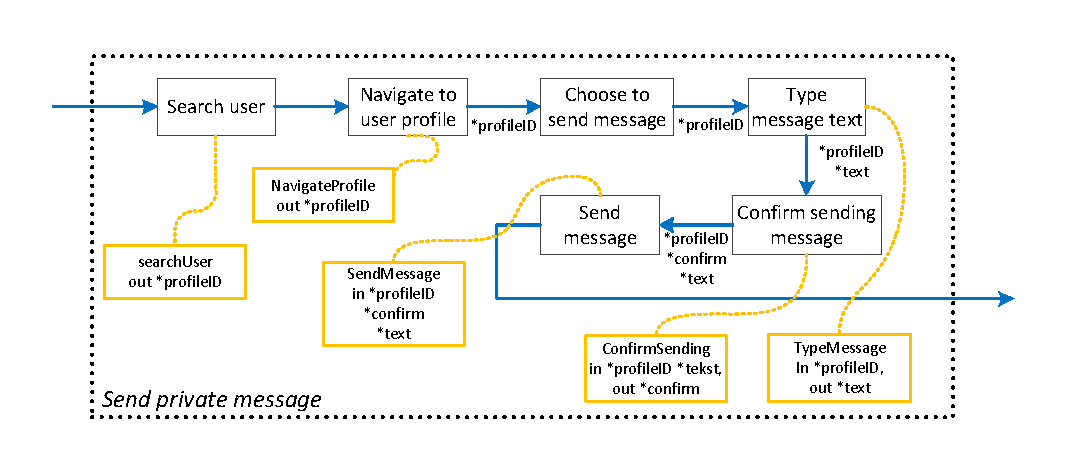
\includegraphics[scale=1]{nav_SendPrivateMessage.pdf}
 \captionof{figure}[Send private message]{Send private message.}
\end{minipage}
$\;$ \\ 

\subsection{Like user}

$\;$ \\
\noindent\begin{minipage}{\textwidth}
    \centering
   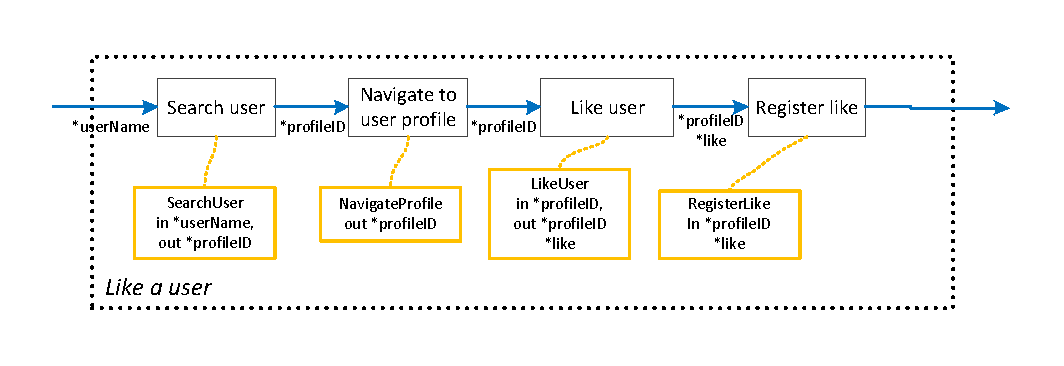
\includegraphics[scale=1]{nav_LikeUser.pdf}
 \captionof{figure}[Like a user]{Like a user.}
\end{minipage}
$\;$ \\ 

\subsection{Manage liked list}

$\;$ \\
\noindent\begin{minipage}{\textwidth}
    \centering
   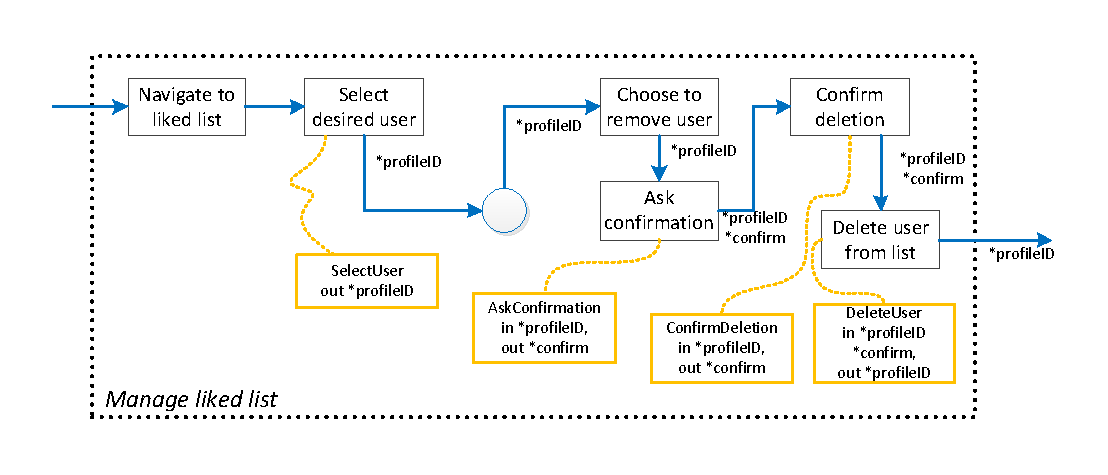
\includegraphics[scale=1]{nav_ManageLikedList.pdf}
 \captionof{figure}[Manage liked list]{Manage liked list.}
\end{minipage}
$\;$ \\ 

\subsection{Notify user in case of profile updates}

$\;$ \\
\noindent\begin{minipage}{\textwidth}
    \centering
   \includegraphics[scale=1]{nav_NotifyProfileUpdate.pdf}
 \captionof{figure}[Notify user of profile updates]{Notify user of profile updates.}
\end{minipage}
$\;$ \\ 

\subsection{Send attention to a user}

$\;$ \\
\noindent\begin{minipage}{\textwidth}
    \centering
   \includegraphics[scale=1]{nav_SendAttention.pdf}
 \captionof{figure}[Send attention]{Sent an attention to the user.}
\end{minipage}
$\;$ \\ 

\subsection{Send private message to a user}

$\;$ \\
\noindent\begin{minipage}{\textwidth}
    \centering
   \includegraphics[scale=1]{nav_SendPrivateMessage.pdf}
 \captionof{figure}[Send private message]{Send a private message.}
\end{minipage}
$\;$ \\ 

\subsection{Block or report a user}

$\;$ \\
\noindent\begin{minipage}{\textwidth}
    \centering
   \includegraphics[scale=1]{nav_BlockReport.pdf}
 \captionof{figure}[Block or report user]{Block or report a user.}
\end{minipage}
$\;$ \\ 

\subsection{Log out}

$\;$ \\
\noindent\begin{minipage}{\textwidth}
    \centering
   \includegraphics[scale=1]{nav_LogOff.pdf}
 \captionof{figure}[Log out]{Log out of the system.}
\end{minipage}
$\;$ \\ 

\subsection{Terminate account}

$\;$ \\
\noindent\begin{minipage}{\textwidth}
    \centering
   \includegraphics[scale=1]{nav_TerminateAccount.pdf}
 \captionof{figure}[Terminate account]{Terminate account.}
\end{minipage}
$\;$ \\ 

\subsection{Display personal information}

$\;$ \\
\noindent\begin{minipage}{\textwidth}
    \centering
   \includegraphics[scale=1]{Nav_DisplayPersonalInformation.pdf}
 \captionof{figure}[Display personal information]{Display personal information.}
\end{minipage}
$\;$ \\ 

\subsection{Display foreign information}

$\;$ \\
\noindent\begin{minipage}{\textwidth}
    \centering
   \includegraphics[scale=1]{Nav_DisplayForeignInformation.pdf}
 \captionof{figure}[Display foreign information]{Display foreign information.}
\end{minipage}
$\;$ \\ 

\subsection{Browse user profile}

$\;$ \\
\noindent\begin{minipage}{\textwidth}
    \centering
   \includegraphics[scale=1]{nav_BrowsUserProfile2.pdf}
 \captionof{figure}[Browse user profile]{Browse user profile.}
\end{minipage}
$\;$ \\ 

\subsection{Send message to any user}

$\;$ \\
\noindent\begin{minipage}{\textwidth}
    \centering
   \includegraphics[scale=1]{nav_SendMessageAnyUser.pdf}
 \captionof{figure}[Send message to any user]{Send message to any user.}
\end{minipage}
$\;$ \\ 

\subsection{Block, disable and delete user account}

$\;$ \\
\noindent\begin{minipage}{\textwidth}
    \centering
   \includegraphics[scale=1]{nav_BlockDisableDelete.pdf}
 \captionof{figure}[Block, disable and delete user account]{Block, disable and delete user account.}
\end{minipage}

\section{Functional Modeling}
%modules

\subsection{Overview of the modules}

An overview of the IFML Modules used for the functionality are depicted in the figure below. Note that these modules do not contain all of the functionalities. Therefore, the reader is invited to also take a look at the Site Structure Design, in section \ref{sec:sitestructure}. \\
Each of the modules is explained in detail in the subsections.

\subsection{Login}

The login module receives an \texttt{password} and \texttt{userName} input parameter that is passed via the input port to the actual login module. The \texttt{password} and \texttt{userName} input parameters are bind to the login module's parameters. In case the login fails, a \texttt{message} as output port parameter is passed to the \texttt{KO Port}.
$\;$ \\ \\
\noindent\begin{minipage}{\textwidth}
    \centering
   \includegraphics[width=\textwidth]{Module_Login.png}
 \captionof{figure}[Login module]{Login logic.}
\end{minipage}
$\;$ \\ 

\subsection{Register new user}

A visitor that wants to create a user account (i.e., to register), has to supply a \texttt{dateOfBirth}, \texttt{description}, \texttt{email}, \texttt{interest}, \texttt{location}, \texttt{password} and \texttt{picture}. These input parameters are bind to the \texttt{CreateUser} module that creates a user in the database with the supplied parameter data. \\
In case of success, the \texttt{password} and \texttt{userName} paramaters are passed to the \texttt{OK Port}. This is because the newly created user is redirected to its profile page.
$\;$ \\ \\
\noindent\begin{minipage}{\textwidth}
    \centering
   \includegraphics[width=\textwidth]{Module_Register.png}
 \captionof{figure}[Register module]{Registration logic.}
\end{minipage}
$\;$ \\ 

\subsection{Logout}

Any registered user that wants to logout can do so by using this module. However, we have to know what user is currently logged on, so the userOid of the currently logged in user is retrieved and passed to the parameter collector. From there, the oid is passed to the actual \texttt{Logout} operation. \\
In case of failure, a message is passed to the output port.
$\;$ \\ \\
\noindent\begin{minipage}{\textwidth}
    \centering
   \includegraphics[width=1.1\textwidth]{Module_Logout.png}
 \captionof{figure}[Logout module]{Log out logic.}
\end{minipage}
$\;$ \\ 

\subsection{Update user profile}

Any registered user can update its profile. Therefore, some profile information has to be supplied: \texttt{dateOfBirth}, \texttt{gender}, \texttt{location}, \texttt{picture} and \texttt{userName}. In addition, the oid of the user is also supplied, because the user is identified by its \texttt{oid} and this value is used to update the user's information in the database. \\
In case of succes, the user is redirected and in case of failure, a message is passed to the output port.
$\;$ \\ \\
\noindent\begin{minipage}{\textwidth}
    \centering
   \includegraphics[width=1.1\textwidth]{Module_UpdateProfile.png}
 \captionof{figure}[Update user profile module]{Logic to update the user's profile.}
\end{minipage}
$\;$ \\ 

\subsection{Delete account}

An administrator is able to delete any user account. The logic is provided by the \texttt{DeleteAccount} operation that receives the user's oid from the input port. This is used to identify the user that is to be deleted. In case of succes or failure, a message is passed to the output port to update the status on the webpage. \\
Because the user oid is passed an input parameter, it is not necessary to retrieve the user oid via a parameter collector.
$\;$ \\ \\
\noindent\begin{minipage}{\textwidth}
    \centering
   \includegraphics[width=1.1\textwidth]{Module_DeleteUser.png}
 \captionof{figure}[Delete user account module]{Logic to delete a user account.}
\end{minipage}
$\;$ \\ 

\subsection{Terminate account}

A single can terminate its own account. However, this time, the user oid is not provided to the input port and has therefore to be retrieved. This is accomplished by the \texttt{GetUser} getter that passed the oid of the currently logged in user to the parameter collector. Then, it is passed to the \texttt{Terminate account} operation, which deletes an account based on the received user oid. \\
In case of success, the user is redirected and in case of failure a message is displayed.
$\;$ \\ \\
\noindent\begin{minipage}{\textwidth}
    \centering
   \includegraphics[width=1.1\textwidth]{Module_Terminate.png}
 \captionof{figure}[Terminate user account module]{Logic to terminate a personal user account.}
\end{minipage}
$\;$ \\ 

\subsection{Send message}

The module below depicts the sending of a (private) message. A message belongs to a user, that's why the user oid needs to be passed to the \texttt{CreateMessage} operation. In addition, each message has a timestamp, so the current time is passed as well. Of course, the message text is supplied as input port parameter as well. \\
In case of success and failure, a message is shown (i.e., passed as output port parameter).
$\;$ \\ \\
\noindent\begin{minipage}{\textwidth}
    \centering
   \includegraphics[width=1.1\textwidth]{Module_SendMessage.png}
 \captionof{figure}[Module to send a private message]{Logic to send a (private) message.}
\end{minipage}
$\;$ \\ 

\chapter{Implementation design}


\section{Site structure design}
\label{sec:sitestructure}


\chapter{Presentation design}

\section{Style and template design}



\newpage

\bibliographystyle{apalike}
\bibliography{WebEngineering}
\addcontentsline{toc}{chapter}{Bibliography}
\end{document}